\documentclass[1pt]{article}
\usepackage {tikz}
\usetikzlibrary {arrows,automata}
\usepackage{amssymb}
\usepackage{listings}
%block scheme
\usepackage{pdfpages}
\usepackage{caption}
%preamble
\usepackage[nottoc]{tocbibind}
\usepackage[T1]{fontenc}
%syllabus check
\usepackage[italian]{babel}
\usepackage{graphicx}


\usepackage{amsmath}

\def\X#1{$#1$ &\tt\string#1}
\newcommand\tab[1][1cm]{\hspace*{#1}}

\makeatletter
\let\@fnsymbol\@arabic
\makeatother
\title{\huge \textrm{Antennas and Coverage}}
\date{\textrm{Politecnico di Milano, \\5 November 2018}}


\begin{document}

	\pagenumbering{gobble}
	\begin{titlepage}
		\maketitle
	\end{titlepage}

	\pagenumbering{arabic}

	\newpage

\centerline{\textbf{Problem}}
A telecommunication company has to install some antennas to cover a region. The region in divided into a set of zones Z. The company can install antennas in a set of candidate sites S. Given a candidate site $i \in S$ and a zone $j \in Z$ it is known the level of the received signal $p_{ij}$. A zone can be served by at most one active antenna and the signal received from that antennas must be greater or equal than $\Delta$.
\\\\
Formulate the problem of maximizing the number of served zones as a linear optimization problem.
\\\\
\textbf{Variant:} In order to avoid poor quality solutions, the company has to introduce constraints on the interference. If a zone j is served by one antenna i, the total of the received signals (minus that of the antenna serving the zone) must be less than or equal to $\delta$.\\\\\\
I modeled the problem in a way that could be solved using AMPL.\\\\
\textbf{Parameters and sets:}\\\\
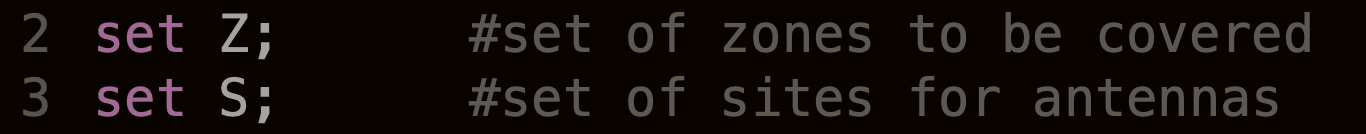
\includegraphics[scale=0.25]{images/sets}\\
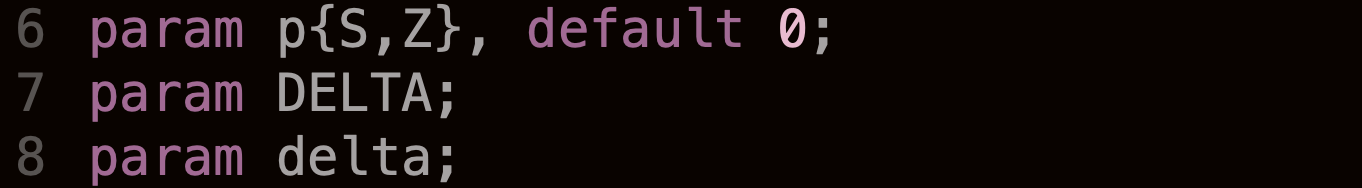
\includegraphics[scale=0.25]{images/params}
\\\\
\textbf{Variable Sets,} Indicate the indexes and their range, the meaning of the variables and their nature (binary, integer...):\\\\
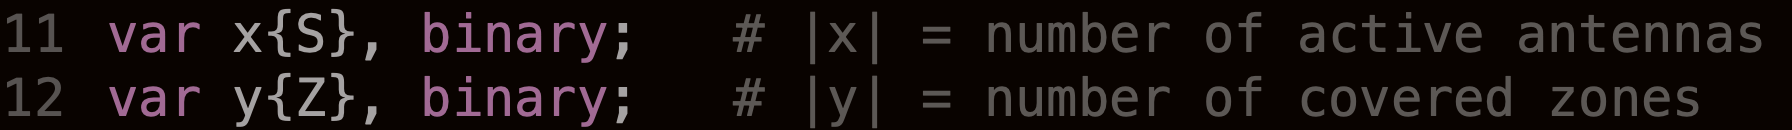
\includegraphics[scale=0.25]{images/variables}
$x_i = 1$ if the antenna is active on site $i$.\\
$x_i = 0$ if the antenna is not active on site $i$.\\
$y_j = 1$ if zone $j$ is covered by some antennas.\\
$y_j = 0$ if zone $j$ is not covered by any antenna.\\
\\\\\\\\\\\\\\
\textbf{Objective function:}\\\\

\includegraphics[scale=0.25]{images/function}
\\\\
\textbf{Constraints about each zone being served by at most one antenna:}\\\\

\includegraphics[scale=0.25]{images/one_antenna}\\
There can not be more than one active antenna that serves each zone.\\\\
\textbf{Constraints about signal quality:}\\\\

\includegraphics[scale=0.25]{images/signal}\\
Each zone is served only if there is an antenna that transmits a signal greater or equal than $\Delta$.\\\\
\textbf{Other constraints if needed:}\\\\
No other constraint is required.\\\\\
\textbf{Constraints of the variant:}\\\\
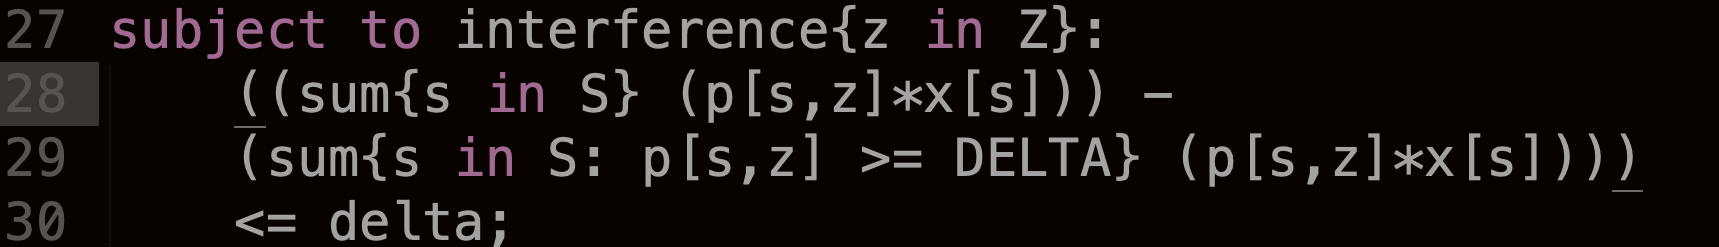
\includegraphics[scale=0.25]{images/variant}\\
Literally, the sum of all the signals received by each zone minus the signal of the antenna that serves the zone must be less or equal than $\delta$.\\\\


\end{document}